% Teilauswertung 2

\newpage
\section{Konzentrationsabhängigkeit von Schichtdicken}
\label{sec:konzDicke}

\begin{center}
	\captionsetup{type=figure}
	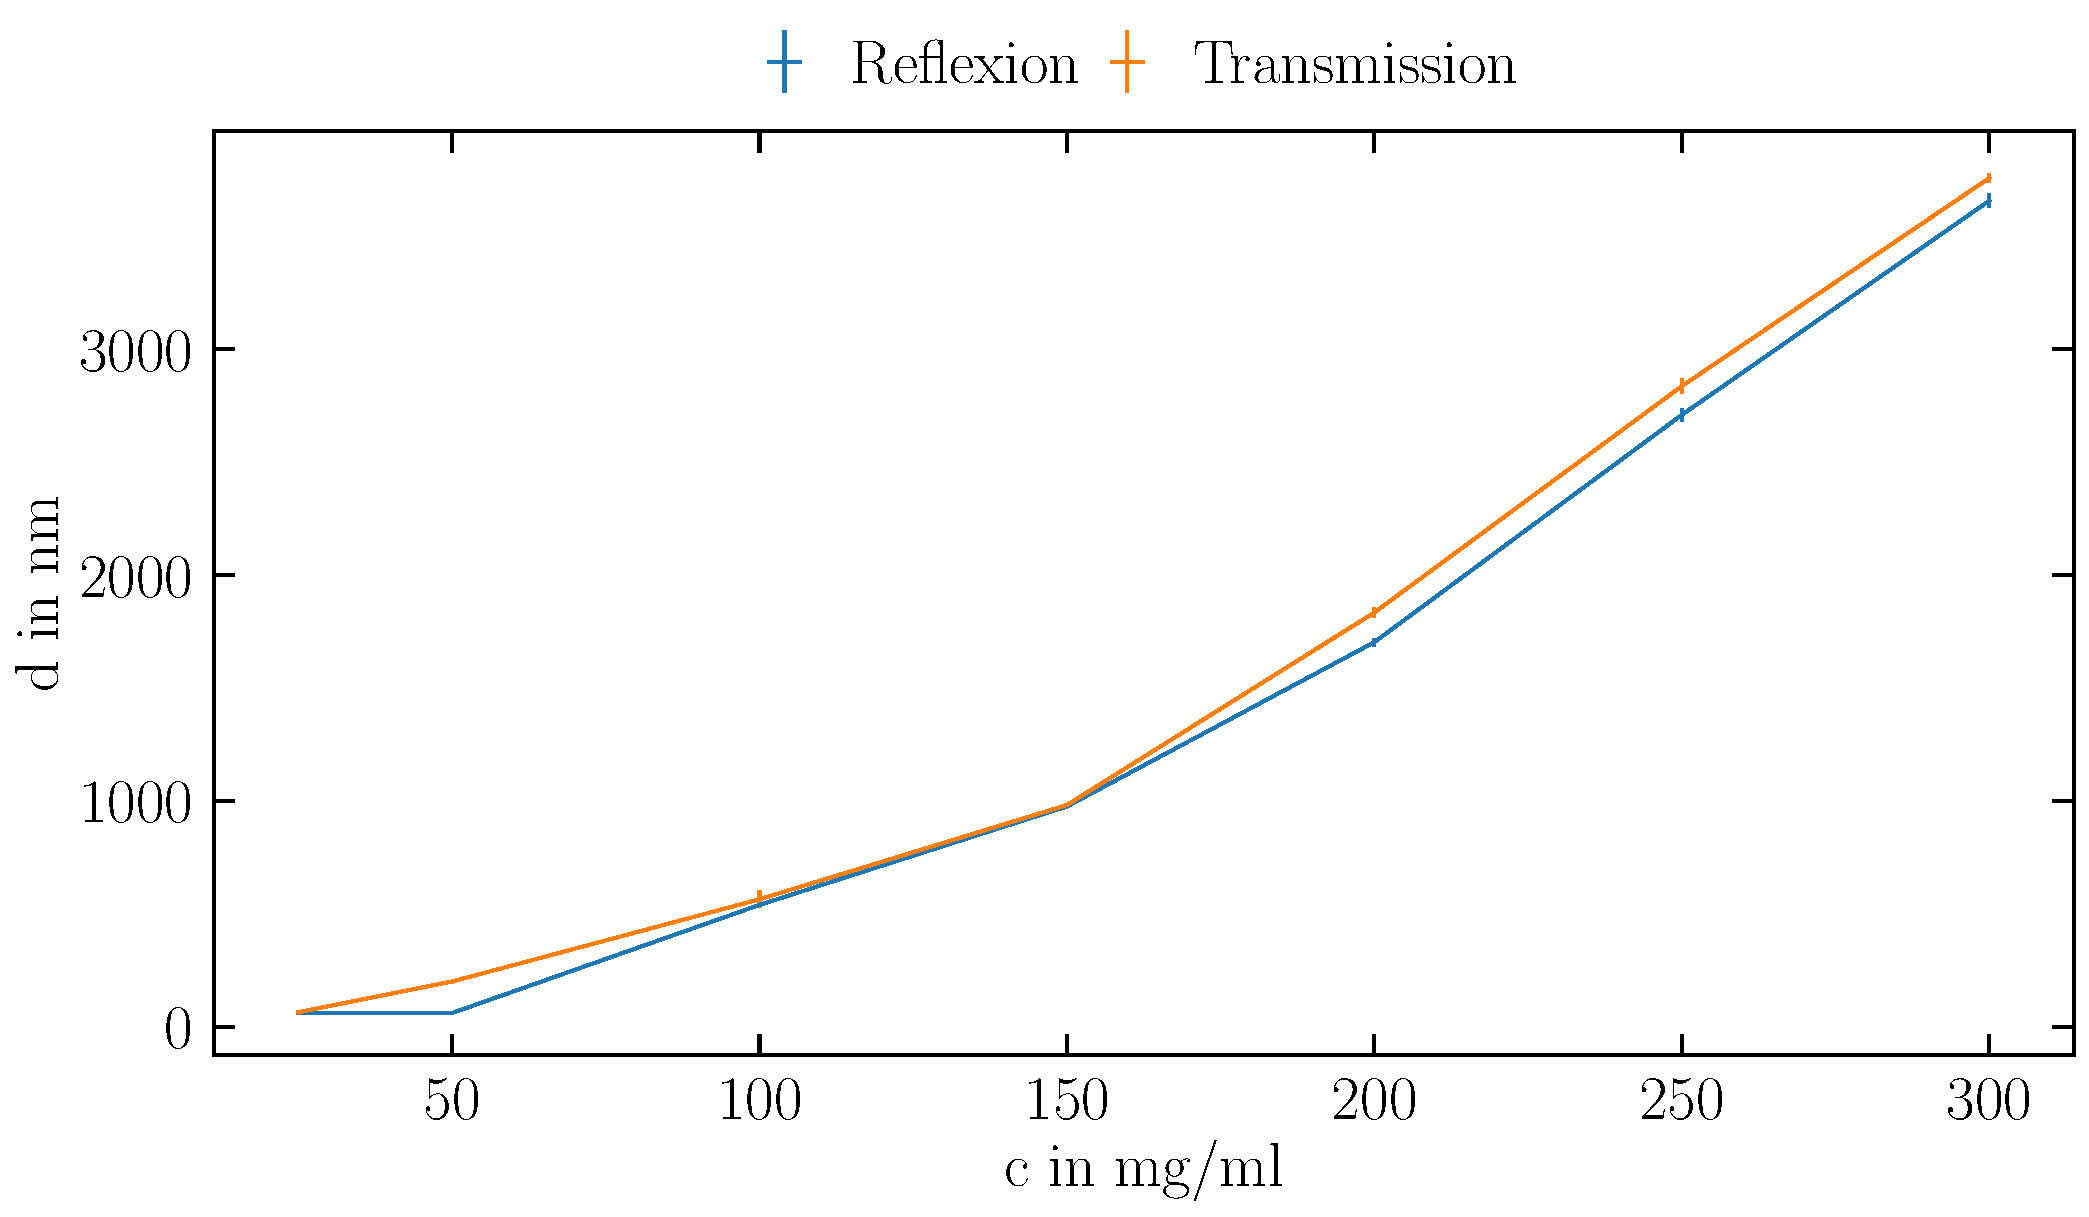
\includegraphics[width=0.92\textwidth]{Auswertung/43/Schichtdicken-Beide.pdf}
	\captionof{figure}{Schichtdicken $d$ der Proben in Abhänigkeit von der Konzentration der Polymerlösung $c$.}
	\label{fig:fitgueteReflexion}
\end{center}


\newpage
\subsection{Bestimmung der kritischen Überlapp-Konzentration $c_0$}

\begin{center}
	\captionsetup{type=figure}
	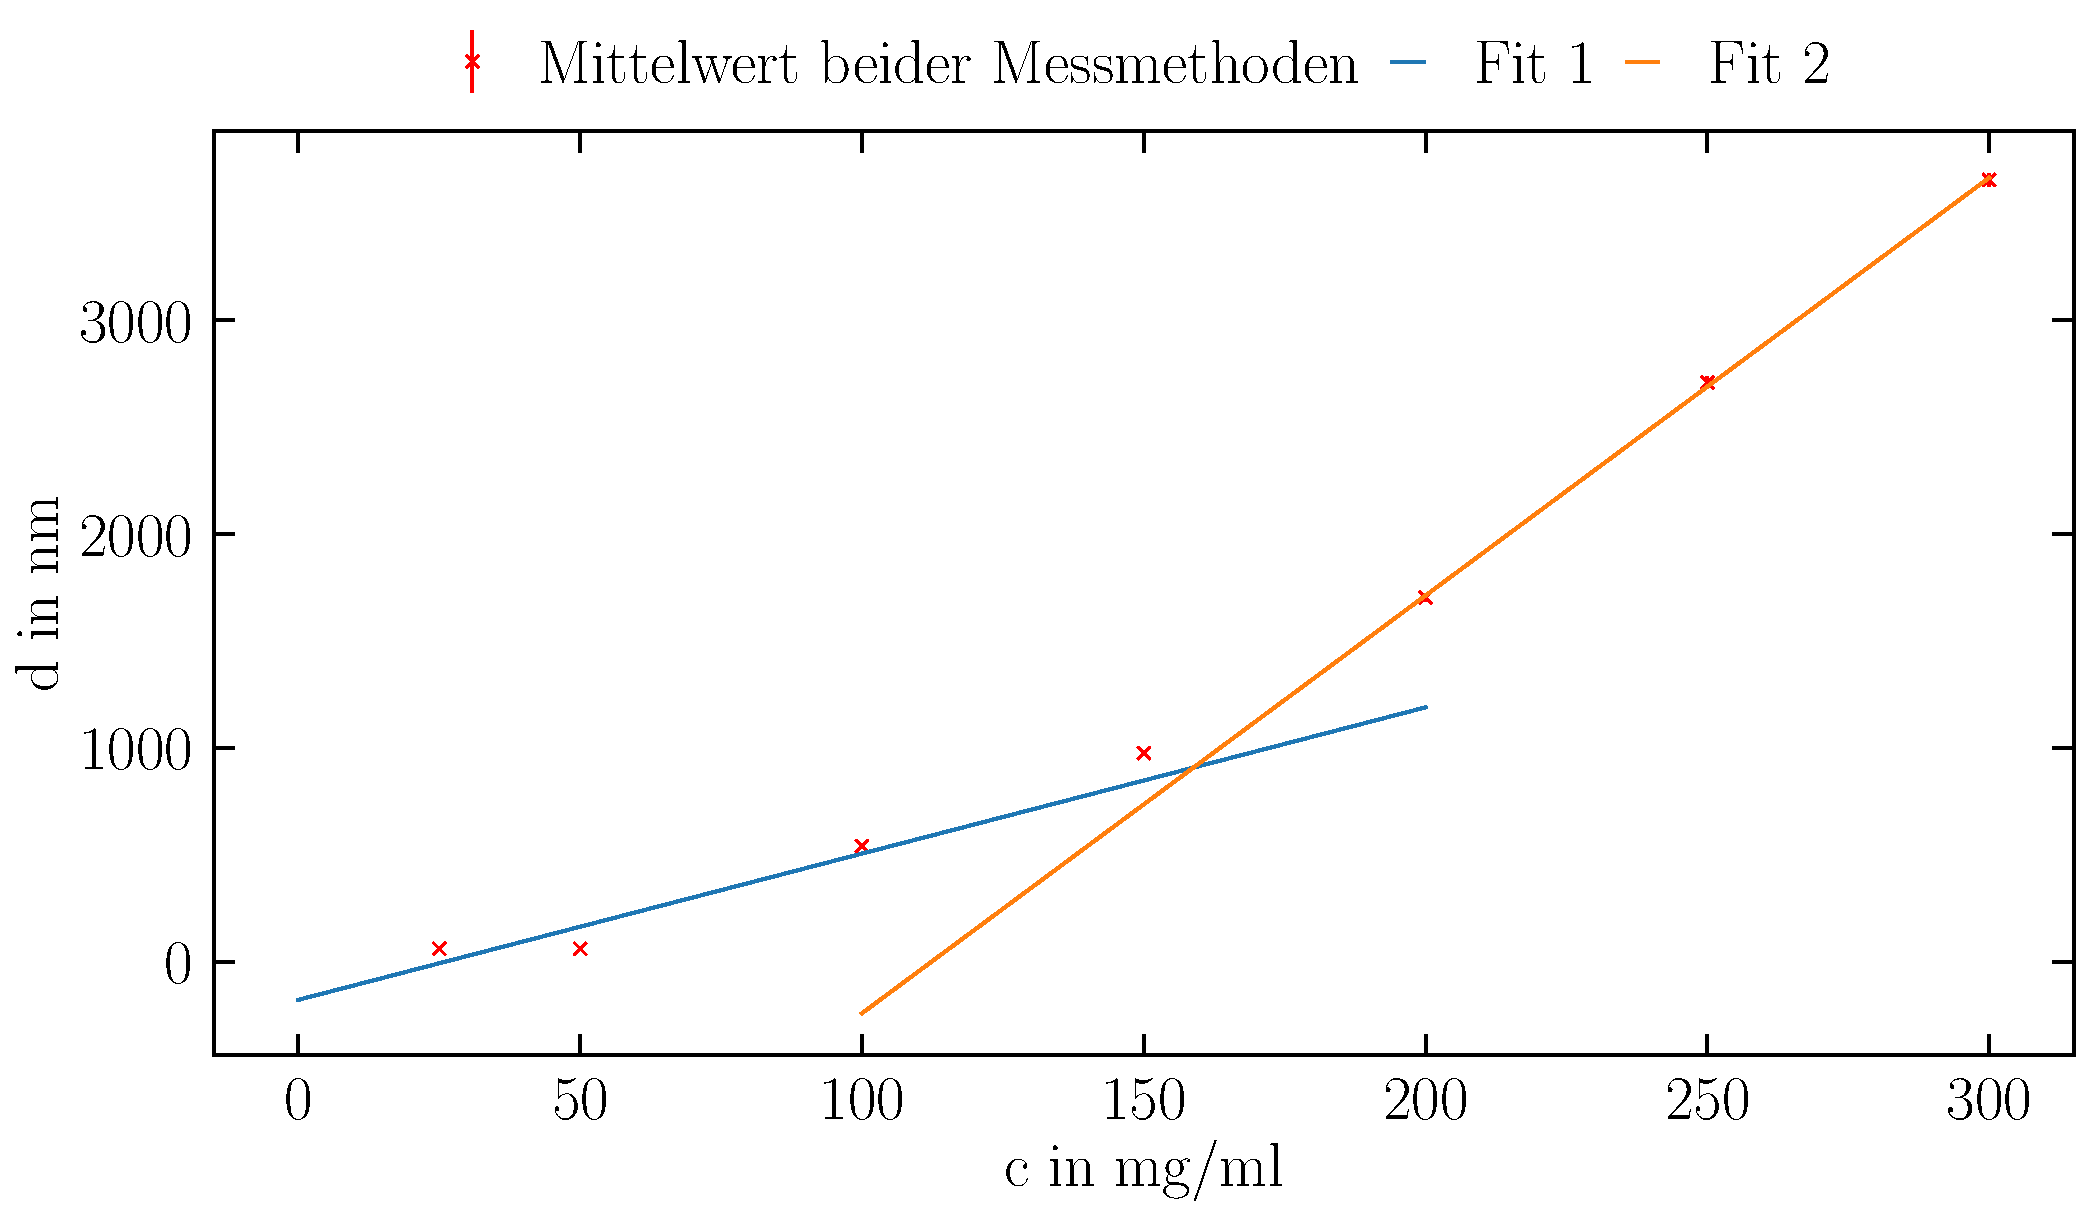
\includegraphics[width=0.92\textwidth]{Auswertung/43/Schichtdicken-Fit.pdf}
	\captionof{figure}{Mittelwert der Schichtdicken $d$ der Proben, aus beiden Messwerten, in Abhänigkeit von der Konzentration der Polymerlösung $c$. Und lineare Fits zur ermittelung der kritischen Überlapp-Konzentration $c_0$.}
	\label{fig:fitgueteReflexion}
\end{center}


\subsection{Berechnung der root-mean-square end-to-end distance}


\subsection{Vergleich der Messdaten mit den bekannten Polymer Modellen}